\textbf{Задача о рюкзаке}\\

$\mathsf{KNAPSACK} = \{  (n_1,..., n_k, m_1.., m_k, N, M): \exists \alpha \in \{0,1\}^k \sum \alpha_in_i \leq N$ и $\sum \alpha_im_i \geq M\}$\\
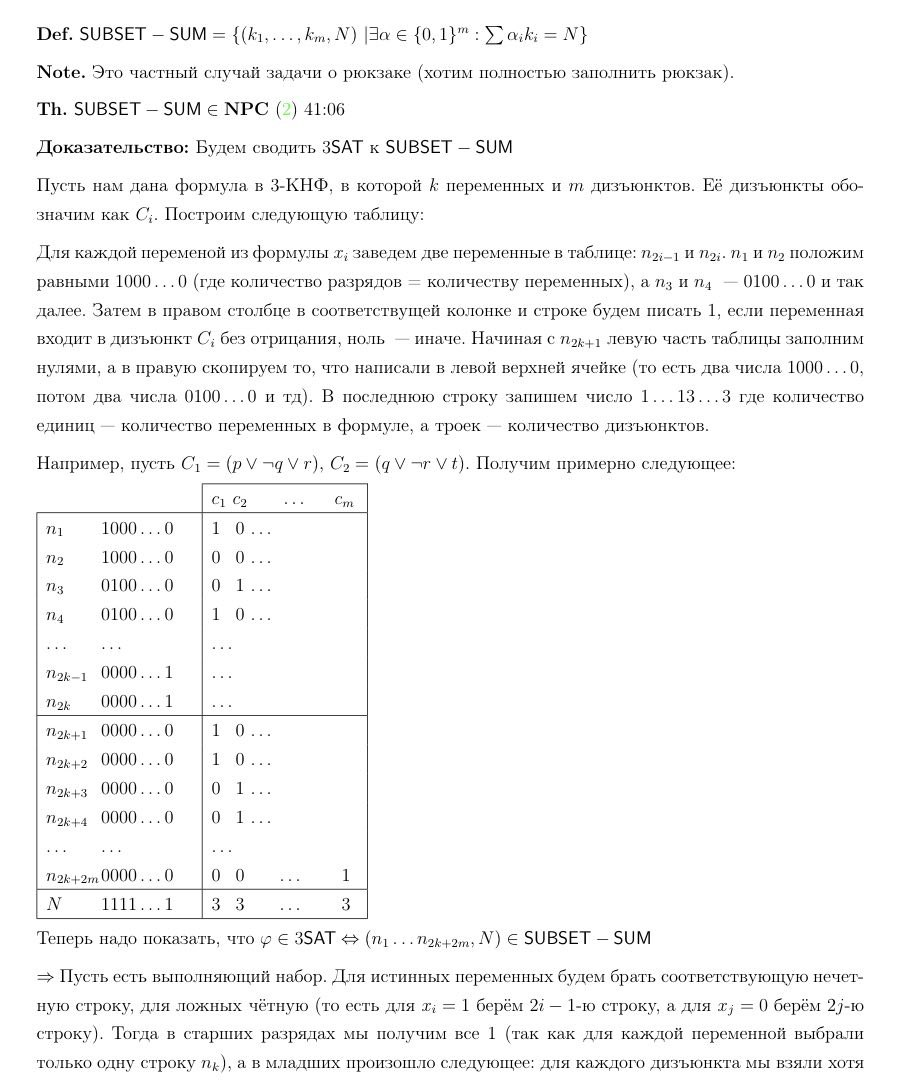
\includegraphics[width=19cm]{images/6_1.jpg}
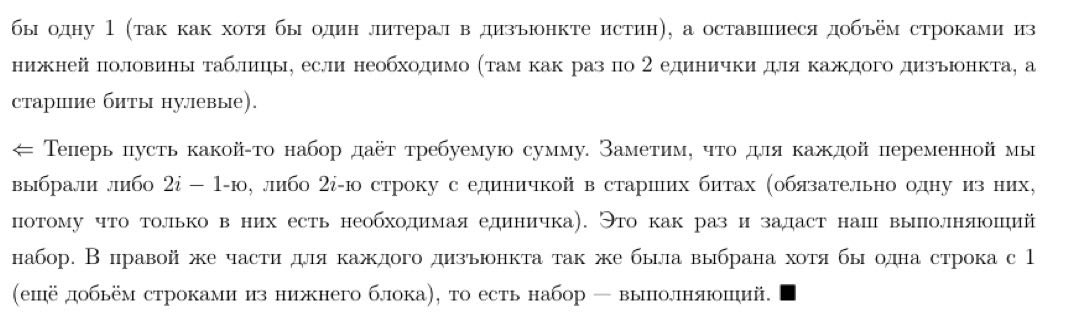
\includegraphics[width=19cm]{images/6_2.jpg}
\textbf{Задача целочисленного программирования}
\\
$\mathsf{INTPROG} = \{A \in Z^{n+m}, \ b\in \Z^n: Ax \leq b$ имеет решение в целых числах$\}$
\begin{theorem}
$\mathsf{INTPROG} \in \npc$
\end{theorem}
\begin{proof}
Для проверки принадлежности к \textbf{NP} достаточно в качестве сертификата передавать решение, тогда нам нужно проверить целочисленность и удовлетворение неравенству. Единственная проблема заключается в том, чтобы доказать полиномиальность сертификата. Это остаётся без доказательства.

Сведем $\mathsf{3SAT}$ к $\mathsf{INTPROG}$. Каждому дизъюнту вида $(p \vee \bar q \vee r)$ сопоставим $$p + (1 - q) + r \geq 1, 0 \leq p,\ q \leq 1.$$ Тогда, если $\phi$ --- выполнима, в качестве решения подойдет выполняющий набор. Если же мы нашли решение, то в силу того, что $q$ и $1 -q$ не могут быть одновременно равны 1, решение будет давать выполняющий набор.
\end{proof}
